\documentclass{article}

% Packages
\usepackage{amsmath, amssymb}
\usepackage[a4paper,top=1.25cm,bottom=1.25cm,left=2.5cm,right=2.5cm,includefoot]{geometry}
\usepackage{graphicx}
\usepackage{hyperref}
\usepackage{adjustbox}
\usepackage{tabularx}
\usepackage[T1]{fontenc}
\usepackage{fancyhdr}
\usepackage{lastpage}
\usepackage{float}
\usepackage{xcolor}
\usepackage{lmodern}
\usepackage{titlesec}

% Color
\definecolor{oceangreen}{HTML}{004b5a}

% Header/Footer
\pagestyle{fancy}
\fancyhf{}
\fancyfoot[L]{\footnotesize\sffamily Medical Robotics CS4270 -- Assignment Submission}
\fancyfoot[C]{\footnotesize\sffamily \thepage\ of \pageref*{LastPage}}
\fancyfoot[R]{\footnotesize\sffamily Exercise Sheet \sheet, Group \groupnumber}
\renewcommand{\headrulewidth}{0pt}

% Section formatting
\titleformat{\section}{\color{oceangreen}\Large\bfseries\sffamily}{\thesection.}{1em}{}
\titleformat{\subsection}{\color{oceangreen}\large\bfseries\sffamily}{\thesubsection.}{1em}{}

% Custom Fields
\newcommand{\groupnumber}{8}
\newcommand{\groupmembers}{Donuru Umakanth Reddy (802457), Alina Khan (819206), Chang Quoc Toan (810588)}
\newcommand{\sheet}{8}
\newcommand{\term}{Summer 2026}

\hypersetup{colorlinks=true, linkcolor=black, urlcolor=black}

\begin{document}

% Header
\noindent
\begin{minipage}[t]{0.6\textwidth}
    \large\sffamily \textcolor{oceangreen}{Medical Robotics CS4270 - Assignment Submission}\\
    \small \term\\
    \small Exercise Sheet \sheet\\
    \small Group \groupnumber\\
    \small \groupmembers
\end{minipage}
\hfill
\begin{minipage}[t]{0.35\textwidth}
    \raggedleft
    
\includegraphics[width=5cm]{logo-rob-eng.png}
\end{minipage}

\vspace{3mm}
{\color{oceangreen}\rule{\linewidth}{0.75pt}}

\footnotesize
Please upload your solutions via the submission activity in the Medical Robotics Moodle course. Submissions must include the names of all group members and be uploaded as a \texttt{.pdf} file.

{\color{oceangreen}\rule{\linewidth}{0.75pt}}
\normalsize

\section {Motion Correlation I}

\subsection{1.A}
\begin{figure}[H]
    \centering
    \setlength{\fboxsep}{6pt} % Padding inside the box
    \setlength{\fboxrule}{0.5pt} % Thickness of the box border
    \fbox{%
        \begin{adjustbox}{max width=0.95\linewidth}
            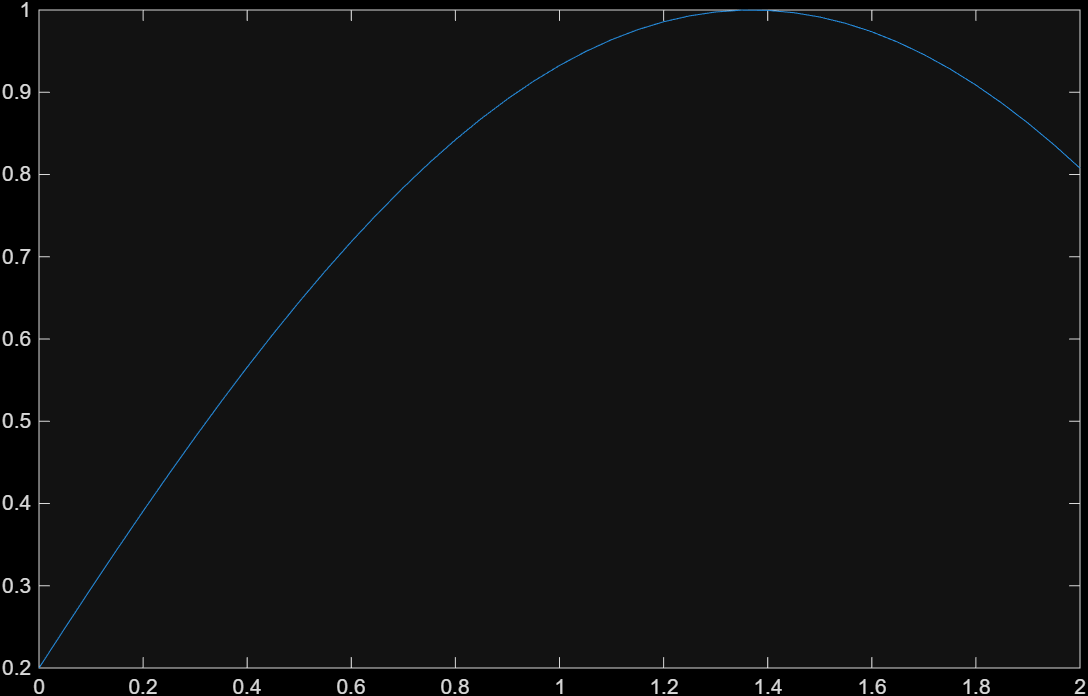
\includegraphics{Figure_1.png}
        \end{adjustbox}%
    }
    \caption{Patient positions plotted over time.}
    \label{fig:patient_positions}
\end{figure}

\subsection{1.B - 1.D}
\begin{figure}[H]
    \centering
    \setlength{\fboxsep}{6pt}
    \setlength{\fboxrule}{0.5pt}
    \fbox{%
        \begin{adjustbox}{max width=0.95\linewidth}
            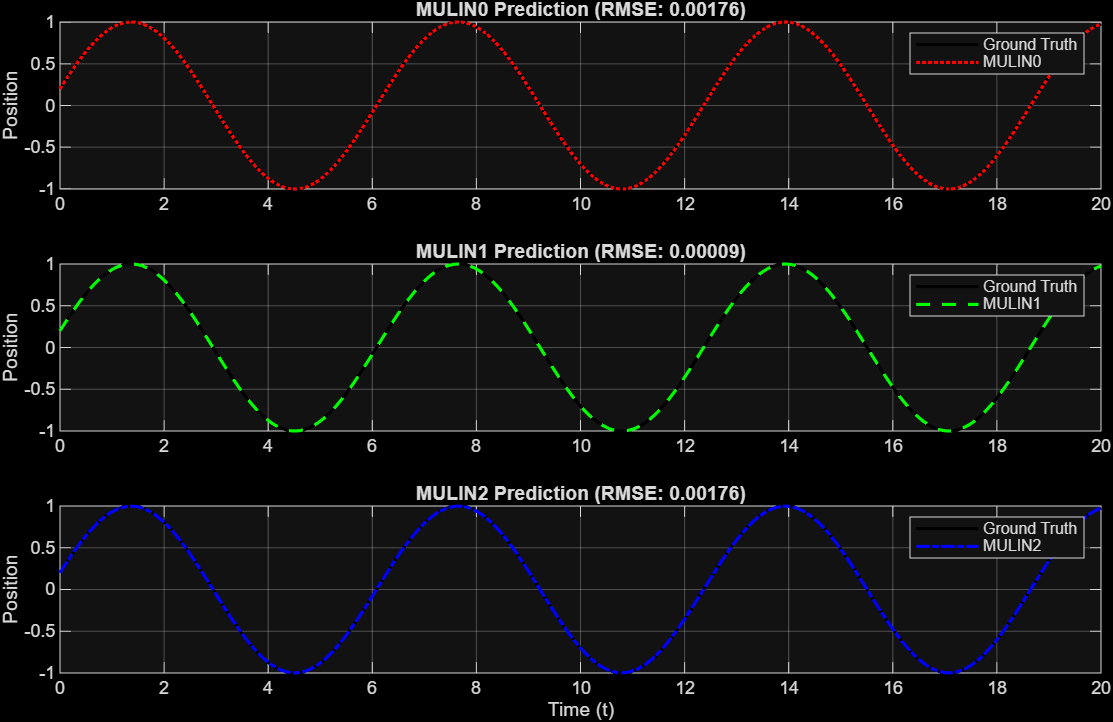
\includegraphics{Figure_2.png}
        \end{adjustbox}%
    }
    \caption{Comparison of MULIN prediction models against ground truth.}
    \label{fig:mulin_comparison}
\end{figure}

\subsection{1.E}
\begin{verbatim}
Console Output:
RMSE for MULIN0: 0.00176229
RMSE for MULIN1: 0.00008806
RMSE for MULIN2: 0.00176230
\end{verbatim}
Observing the RMSE values, it is clear that the MULIN order 1 is the best for the following case.

\section{Least Mean Squares}
\subsection{2.A}
\begin{figure}[H]
    \centering
    \setlength{\fboxsep}{6pt}
    \setlength{\fboxrule}{0.5pt}
    \fbox{%
        \begin{adjustbox}{max width=0.95\linewidth}
            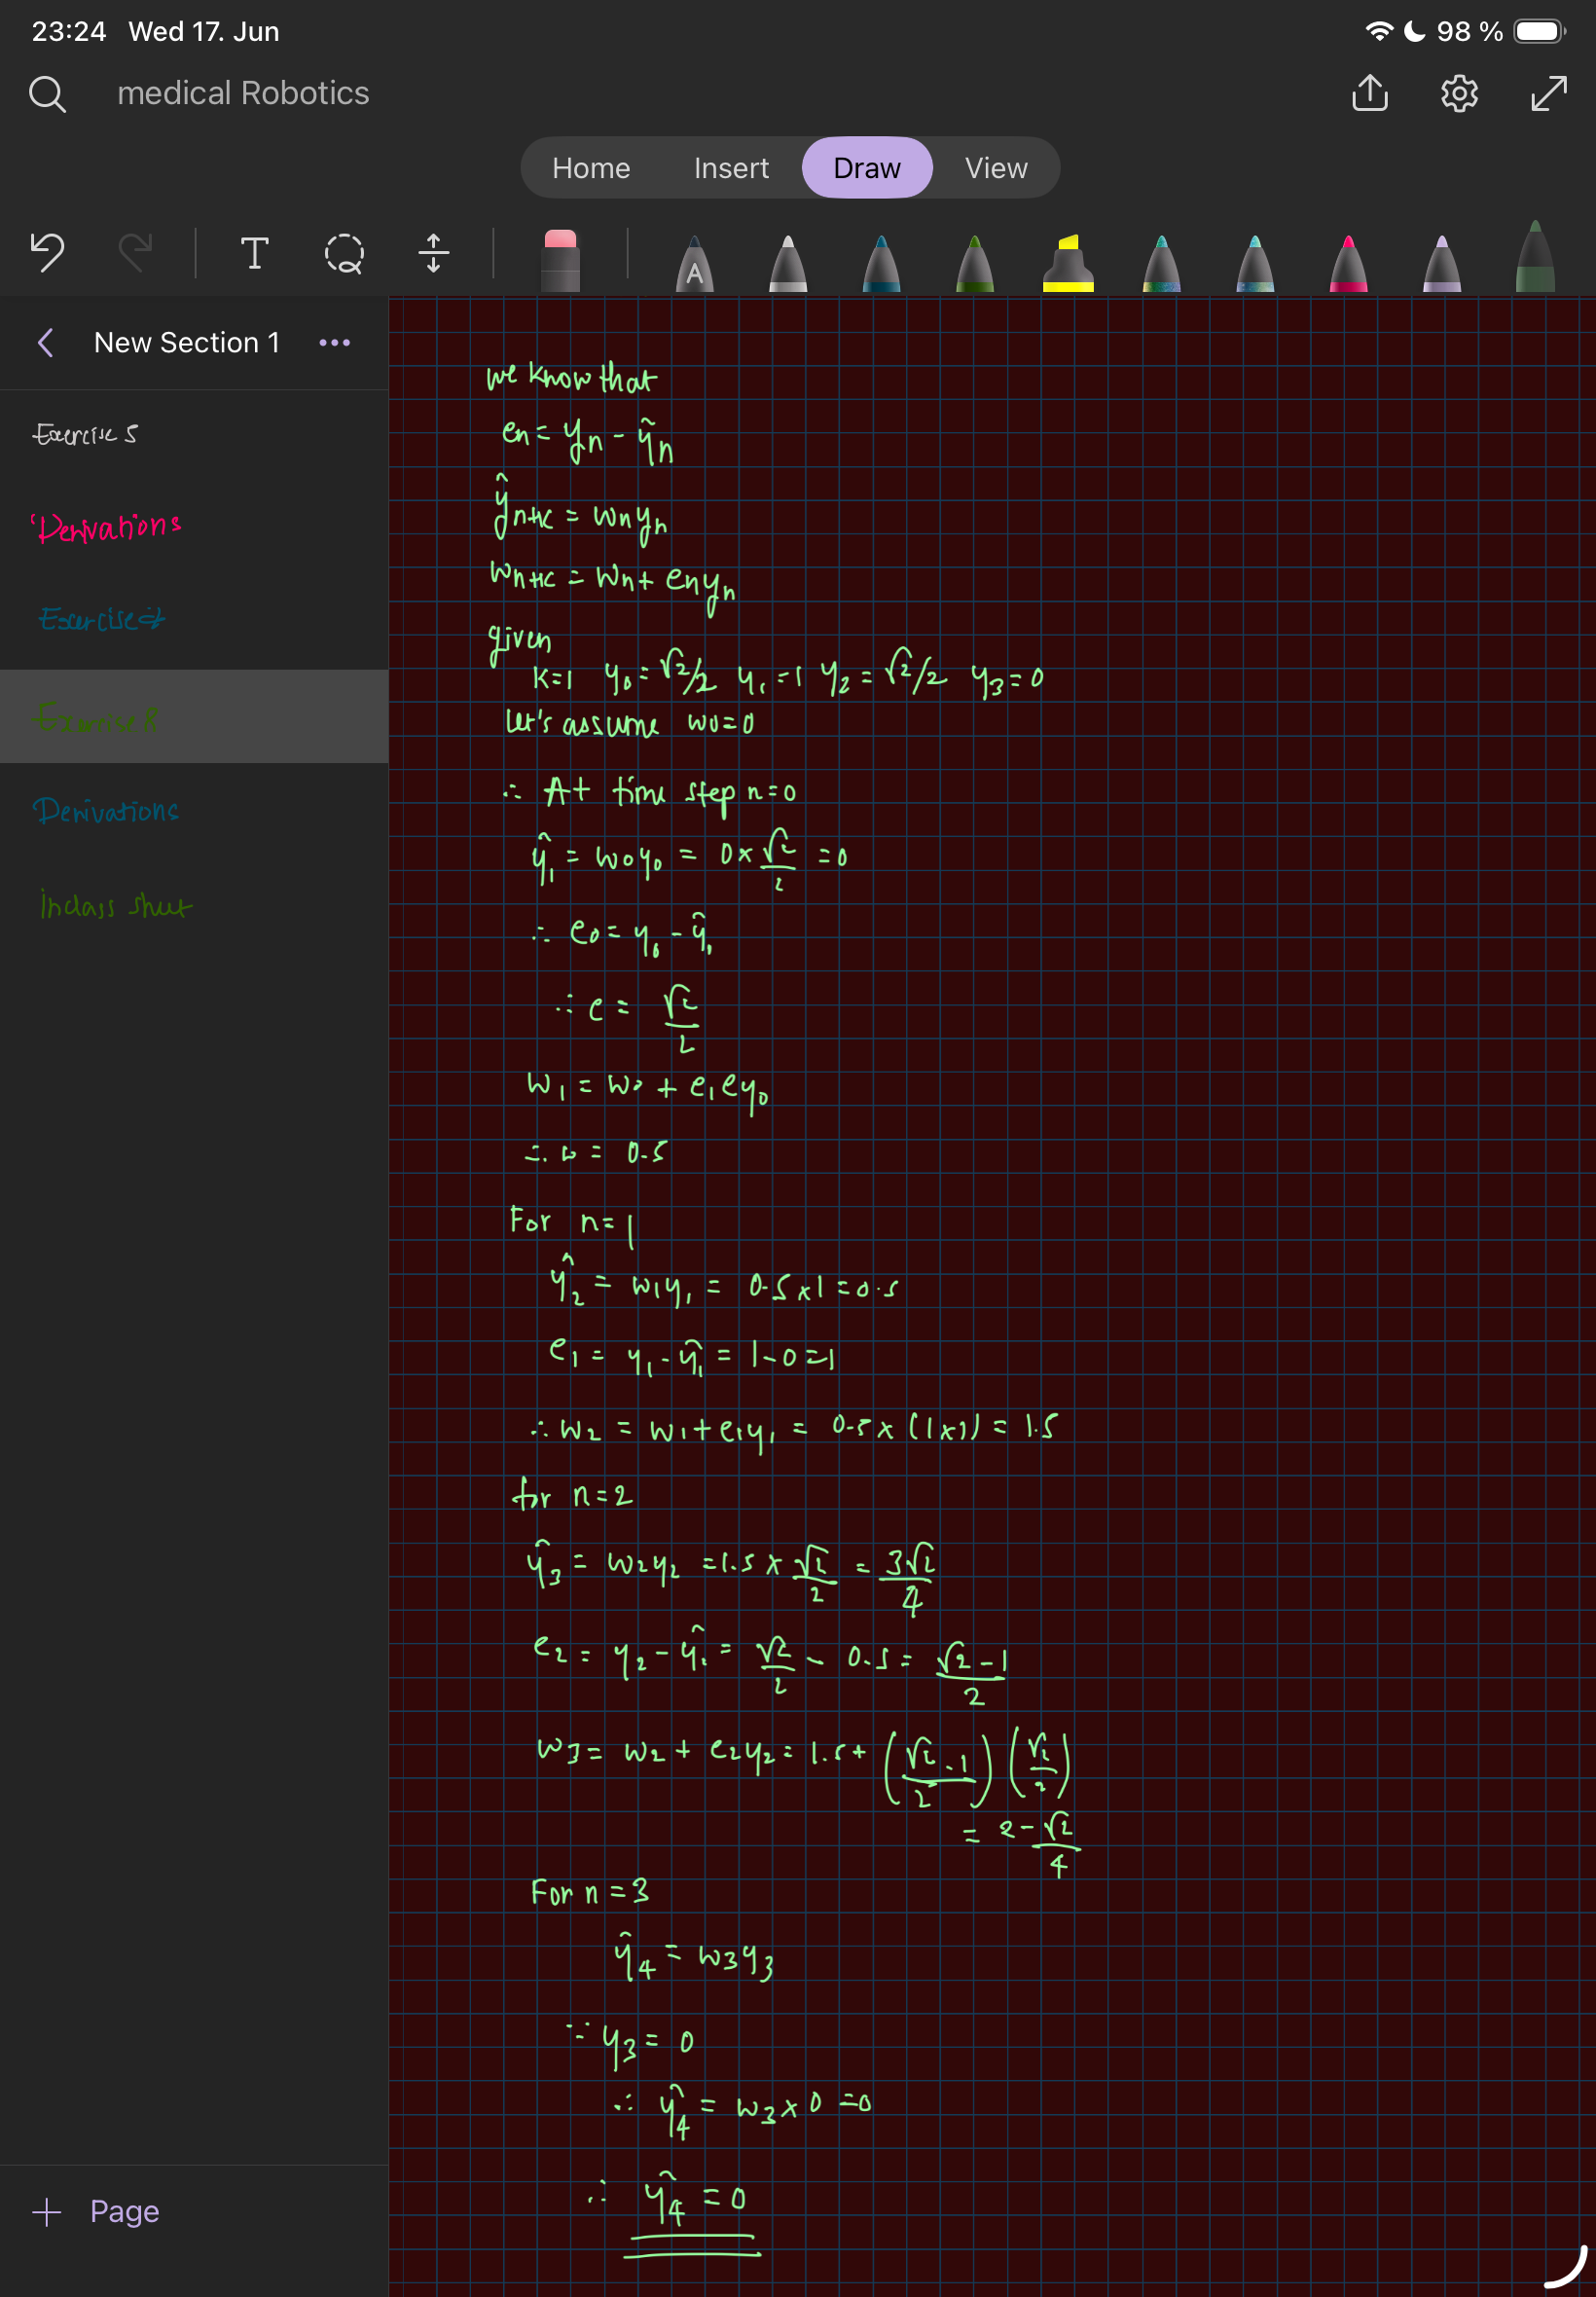
\includegraphics{IMG_0105.png}
        \end{adjustbox}%
    }
    \caption{Calculation of $\hat{y}_4$ using the LMS algorithm.}
    \label{fig:pen_paper_solution}
\end{figure}

\subsection{2.B}
\begin{figure}[H]
    \centering
    \setlength{\fboxsep}{6pt}
    \setlength{\fboxrule}{0.5pt}
    \fbox{%
        \begin{adjustbox}{max width=0.95\linewidth}
            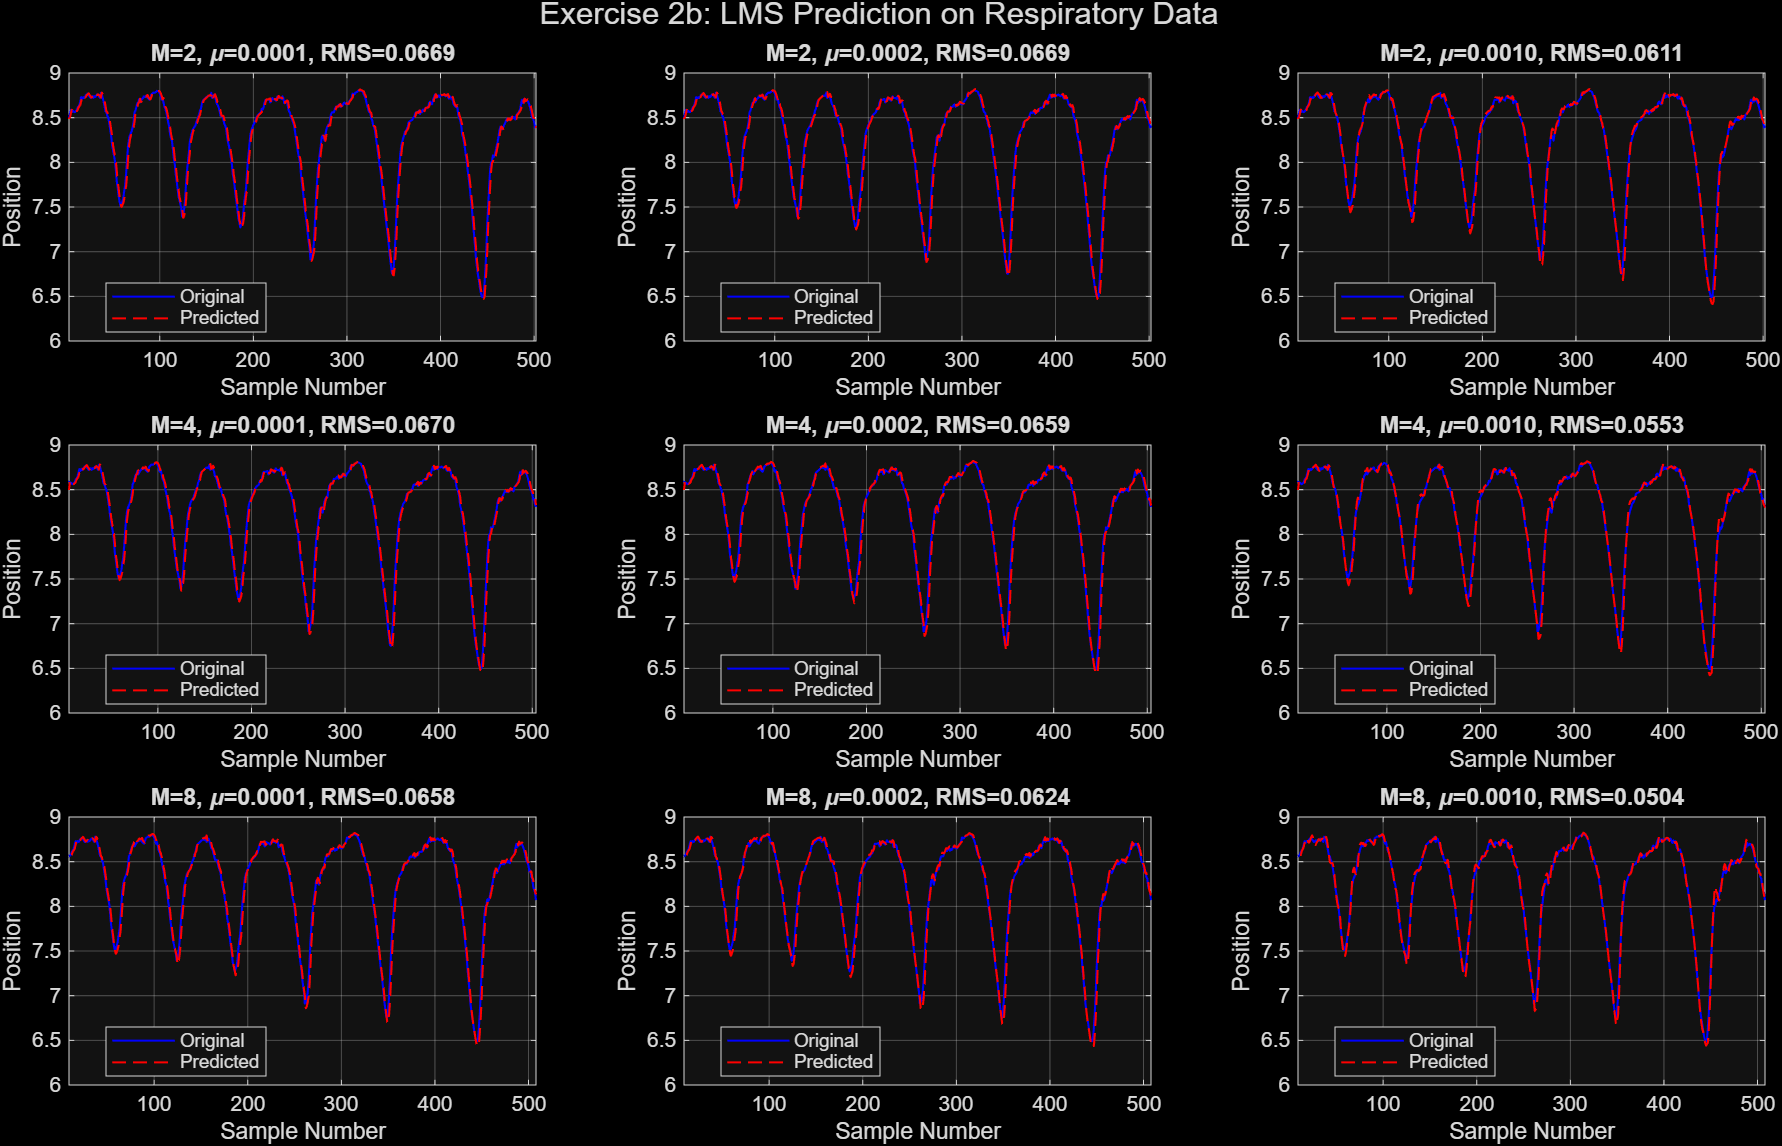
\includegraphics{LMS Predictions - All Combinations.png}
        \end{adjustbox}%
    }
    \caption{All the Plots wrt y, M and u.}
    \label{fig:LMS Predictions}
\end{figure}

\subsection{2.C}
\begin{verbatim}
========== LMS RESULTS ==========
   M   |    mu    |     RMS
--------------------------------
   2   |  0.0001   |   0.066892
   2   |  0.0002   |   0.066931
   2   |  0.0010   |   0.061117
   4   |  0.0001   |   0.066981
   4   |  0.0002   |   0.065891
   4   |  0.0010   |   0.055339
   8   |  0.0001   |   0.065843
   8   |  0.0002   |   0.062422
   8   |  0.0010   |   0.050442
--------------------------------
BEST: M=8, mu=0.0010, RMS=0.050442
================================
\end{verbatim}

As the console output shows the value of RMSE decreases as the value of M and $\mu$ increases, This is due to the algorithm having access to more data points.
\end{document}
